\documentclass{beamer}
\setbeamertemplate{navigation symbols}{}

\usepackage[english]{babel}
\usepackage{array}
\usepackage{listings}
\usepackage{color}
\usepackage{hyperref}
\usepackage{trace}
\usepackage[scriptsize]{caption}

\usepackage{tikz}
\usetikzlibrary{arrows,shapes,positioning,calc}

\usetheme{Boadilla}

%\setbeamertemplate{footline}
%{
%  \leavevmode
%  \hbox{
%    \begin{beamercolorbox}[wd=.5\paperwidth,ht=2.5ex,dp=1.125ex,leftskip=.3cm,rightskip=.3cm plus1fil]{author in head/foot}
%      \usebeamerfont{author in head/foot}\insertshortauthor \hfill \inserttitle
%    \end{beamercolorbox}
%    \begin{beamercolorbox}[wd=.48\paperwidth,ht=2.5ex,dp=1.125ex,leftskip=.3cm,rightskip=.3cm plus1fil]{title in head/foot}
%      \usebeamerfont{title in head/foot}\insertshortdate \hfill \insertframenumber{}/\inserttotalframenumber
%    \end{beamercolorbox}
%  }
%  \vskip0pt
%}

\definecolor{lgray}{rgb}{0.8,0.8,0.8}
\definecolor{dgreen}{rgb}{0.0,0.8,0.0}

\lstset{breakatwhitespace,
language=C,
backgroundcolor=\color{lgray},
%columns=fullflexible,
keepspaces,
breaklines,
tabsize=3, 
frame=shadowbox,
basicstyle=\ttfamily\fontsize{5}{6}\selectfont,
showstringspaces=false,
keywordstyle=\color{blue},
commentstyle=\color{dgreen},
extendedchars=true}

\setbeamercovered{transparent}

\begin{document}
\title[\today]{Verilog\\Open Source and FPGA\\Zynq, Pynq and Alveo}
\author{Mirko Mariotti}
\date{\today}

\begin{frame}
{
    
\includegraphics[width=0.2\textwidth]{mi.png}  
    \hfill
    
\includegraphics[width=0.7\textwidth]{iscs.png}
}
\titlepage
\end{frame}

\begin{frame}\frametitle{Contents}
\fontsize{6}{7.2}\selectfont
\tableofcontents
\end{frame} 

\section{Introduction}

\subsection{Modules}

\begin{frame}\frametitle{Modules}
\begin{itemize}
	\item<1-> Verilog modules are blocks of code (circuit) that can be reused within other blocks (similar to functions in computer programming languages)
	\item<2-> The keyword ``module'' starts a block that ends with ``endmodule''.
	\item<3-> They could have input and output parameters.
	\item<3-> \lstinputlisting[language=verilog]{modexample.v}
\end{itemize}
\end{frame}

\begin{frame}\frametitle{Main Module}
\begin{itemize}
	\item<1-> A specific module is tagged as the main module. (similar to the main on a programming language)
	\vspace{0.5cm}
	\item<2-> It is the ``program'' entry point.
	\vspace{0.5cm}
	\item<3-> Usually it has inputs and outputs connected to FPGA physical IO.
\end{itemize}
\end{frame}

\subsection{Blocks}

\begin{frame}\frametitle{Blocks}
The verilog block are defined with begin - end. \\
\pause
\vspace{0.3cm}
There are two types of blocks: \\
\pause
\vspace{0.3cm}
\textbf{Initial block} \\
Is executed when the simulation start or as initial value. \\
\pause
\vspace{0.3cm}
\textbf{Always block} \\
It is always executed and is associated to a list that specify when execute the block \\
\lstinputlisting[language=verilog]{always.v}
\end{frame}

\subsection{Data}



\begin{frame}\frametitle{Data}\framesubtitle{Wire e Reg}
\textbf{Wire}:\\
They are used to connect different elements. They can be thought as physical wires. They can be read or assigned but they does not store information. 
Indeed they need to be continuously driven from an assignment or a module port. \\
\vspace{1cm}
\textbf{Reg}:\\
Store a value in Verilog. The value is kept until assigned again (similar to a variable) \\
\end{frame}

\begin{frame}\frametitle{Numbers}
The generic number value in Verilog is: \\
\textless size\textgreater \lq \textless base\textgreater \textless value\textgreater \\
\vspace{0.5cm}
Esempi: \\
12 // decimal (base 10) \\
8 \lq h5F // hexadecimal, 8 bit \\
6 \lq b11\_0010 // binary,  6 bit \\
\lq o576 // octal with no dimension \\
32 \lq bz // binary a 32 bit Hi-Z \\
\vspace{0.3cm}
The char \_ is ignored and can be used as separator.
\end{frame}

\begin{frame}\frametitle{Scalars and Vectors}
Variable can be scalar or vectors. \\
\vspace{0.3cm}
Examples: \\
reg out; // scalar \\
reg [7:0] databus; // 8 bit bus \\
wire [1:0] select; // 2 bit bus \\
wire enabled; // scalar
\end{frame}
 	
\begin{frame}\frametitle{Assignment}
	\textbf{(reg) Blocking assignment}: \\
	A = 3; \\
	The expression is evaluated in the execution flux and the variable assigned immediately. \\
	\pause
	\vspace{0.3cm}
	\textbf{(reg) NON blocking assigment}: \\
	A \textless= A + 1; \\
	The expression is evaluated in the execution flux and the result stored in a temporary variable and assigned on the next step \\
	\pause
	\vspace{0.3cm}
	\textbf{(wire) Continuous assignment}: \\
	assign A = in1 \& in2; \\
	used to model combinatorial logic and rename signals.
	
\end{frame}	

\begin{frame}\frametitle{Operators}
\begin{center}
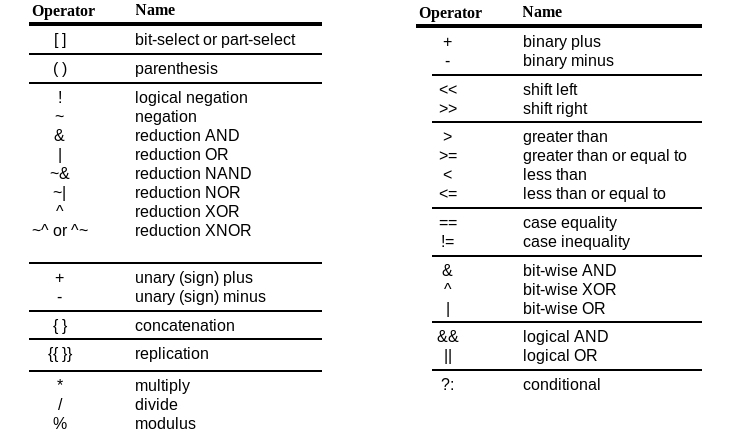
\includegraphics[width=0.9\textwidth]{operatori.jpg}
\end{center}
\end{frame}

\begin{frame}\frametitle{Flow control}\framesubtitle{If-else,  case}
	\lstinputlisting[language=verilog]{ifelse.v}
	\vspace{0.5cm}
	\lstinputlisting[language=verilog]{case.v}
\end{frame}

\begin{frame}\frametitle{Flow control}\framesubtitle{for}
Similar to the C,C++ for loop. no support for ++ \\
\vspace{1cm}
\lstinputlisting[language=verilog]{for.v}
\end{frame}

\section{Live examples}

\begin{frame}\frametitle{Live examples}
\framesubtitle{General informations 1}
You can use either the local installation of Vivado or the cloud infrastructure. \\
\vspace{0.5cm}
\begin{alertblock}{Clone the day3 repository from GitHub}
git clone https://github.com/FPGA-course-2025/day3
\end{alertblock}
or, if you have already cloned the course repository
\begin{alertblock}{Pull the latest changes}
git pull (from inside the day3 folder)
\end{alertblock}
\end{frame}

\begin{frame}\frametitle{Live examples}
\framesubtitle{General informations 2}
Inside the verilog directory in day3 you will find the examples \\
\vspace{0.7cm}
A single example is one or more files with the extension .v or .vhdl
and it's contained in a folder with the example name. \\
\vspace{0.7cm}
You can run the example with Vivado in the following way:
\begin{itemize}
	\item create a new project
	\item add all the files in the project as design sources
	\item add the correct constrains file for the board you are using (also in the day3 verilog directory)
	\item create the bitstream, it should be generated without errors
\end{itemize}
\end{frame}

\begin{frame}\frametitle{Live examples}
\framesubtitle{General informations 3: boards recap}
Basys3:
\begin{itemize}
	\item Part number: xc7a35tcpg236-1
	\item Constraints file: basys3.xdc
\end{itemize}
\vspace{1cm}
Arty 7:
\begin{itemize}
	\item Constraints file: arty7.xdc
\end{itemize}
\end{frame}

\begin{frame}\frametitle{Counter}
\framesubtitle{day3/verilog/counter}
\lstinputlisting[language=verilog]{counter.v}
\vspace{0.5cm}
Let's try some improvements:
\begin{itemize}
	\item Make the counter running faster (or slower)
	\item Add a reset button (with a switch or a button)
\end{itemize}

\end{frame}
\begin{frame}\frametitle{Led on and off}
\framesubtitle{day3/verilog/ledonoff}
\lstinputlisting[language=verilog]{ledonoff.v}
\vspace{0.5cm}
% Let's try some improvements:
% \begin{itemize}
% 	\item Make the counter running faster (or slower)
% 	\item Add a reset button (with a switch or a button)
% \end{itemize}
\end{frame}

\begin{frame}\frametitle{Module instantiation}
\framesubtitle{day3/verilog/modulev}
\lstinputlisting[language=verilog]{modulev.v}
\vspace{0.1cm}
\lstinputlisting[language=verilog]{patternmux.v}
\end{frame}

\begin{frame}\frametitle{VHDL module instantiation}
\framesubtitle{day3/verilog/modulevhdl}
\lstinputlisting[language=verilog]{modulevhdl.v}
\vspace{0.1cm}
\lstinputlisting[language=vhdl]{patternmux.vhdl}
\end{frame}

\section{Open Source and FPGA}

\subsection{Open Source tools for simulation}

\begin{frame}\frametitle{Open Source tools for simulation}
\begin{itemize}
	\item \textbf{iverilog}: a free Verilog simulator, it can be used to simulate the code and check the results.
	\vspace{0.3cm}
	\item \textbf{gtkwave}: a free waveform viewer, it can be used to visualize the results of the simulation.
	\vspace{0.3cm}
	\item \textbf{ghdl}: a free VHDL simulator, it can be used to simulate the VHDL code and check the results.
\end{itemize}
\vspace{0.3cm}
The day3/verilogExamples directory contains a set of 
Jupyter notebooks that can be used to run the examples
with the open source tools.
\vspace{0.3cm}
Similarly, the day3/vhdlExamples directory contains a set
of Jupyter notebooks that can be used to run the VHDL examples with the open source tools.
\end{frame}

\subsection{Open Source tools for synthesis and implementation}

\begin{frame}\frametitle{Open Source tools for synthesis and implementation}
While the major FPGA vendors provide their own synthesis 
and implementation tools, there are also open source alternatives 
that can be used to synthesize and implement designs 
for FPGAs. These tools are particularly useful for 
educational purposes or for those who prefer to work 
with open source software. \\
\vspace{0.5cm}
Related to these tools, there is a growing community of
open source FPGA tools that provide complete flows. Is 
some cases, these tools are better than the vendor tools,
especially for smaller FPGAs or for specific applications. \\
\vspace{0.5cm}
Also the open hardware community is growing, with many
projects that provide open source designs for FPGAs.

\end{frame}

\begin{frame}\frametitle{Open Source tools for synthesis and implementation}

\begin{itemize}
	\item \textbf{Yosys}: a free synthesis tool, it can be used to synthesize the Verilog code and generate a netlist.
	\vspace{0.3cm}
	\item \textbf{nextpnr}: a free place and route tool, it can be used to place and route the netlist generated by Yosys.
	\vspace{0.3cm}
	\item \textbf{icepack}: a free tool to generate the bitstream for Lattice iCE40 FPGAs.
\end{itemize}

\vspace{0.3cm}

A common way to install these tools is to use the
\href{https://github.com/YosysHQ/oss-cad-suite-build/}{
\textbf{oss-cad-suite}} project, which provides
a comprehensive set of open source tools for FPGA design.

\vspace{0.3cm}
The day3/ossExamples directory contains a set of
Jupyter notebooks that can be used to run the examples
with the open source tools and some small FPGAs.

\end{frame}

\section{Zynq, Pynq and Alveo}

\subsection{Zynq}

\begin{frame}\frametitle{Zynq}
Zynq is a family of FPGAs that combines a dual-core ARM Cortex-A9
processor with an FPGA fabric. This allows for a high degree of
integration and flexibility, as the processor can be used to run
software applications while the FPGA fabric can be used to implement
custom hardware accelerators or other logic. \\
\vspace{0.5cm}
\centering
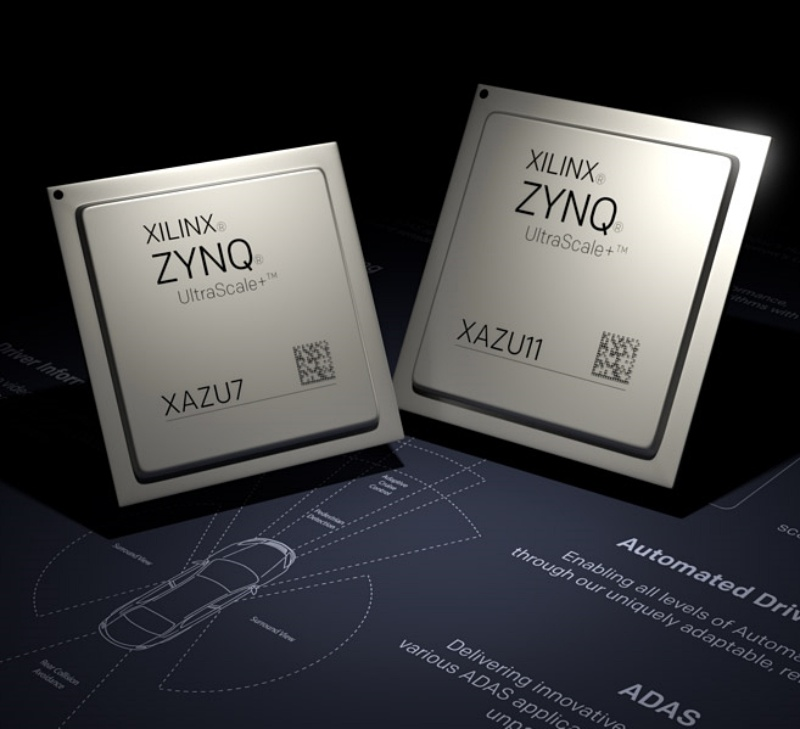
\includegraphics[width=0.4\textwidth]{zynq.jpg}
\end{frame}

\begin{frame}\frametitle{PS-PL}
The Zynq architecture is divided into two main parts:
 the Processing System (PS) and the Programmable Logic 
 (PL). \\
\vspace{0.7cm}
The PS contains the ARM processor, memory controllers,
and other peripherals, while the PL contains the FPGA fabric. \\
\vspace{0.7cm}
The PS can run a standard operating system, such as Linux,
or a real-time operating system like FreeRTOS. \\
\vspace{0.7cm}
The PS and PL can communicate with each other through a set of
interfaces, such as AXI, which allows for high-speed data transfer
between the two parts. \\
\end{frame}

\begin{frame}\frametitle{PS-PL}
\centering
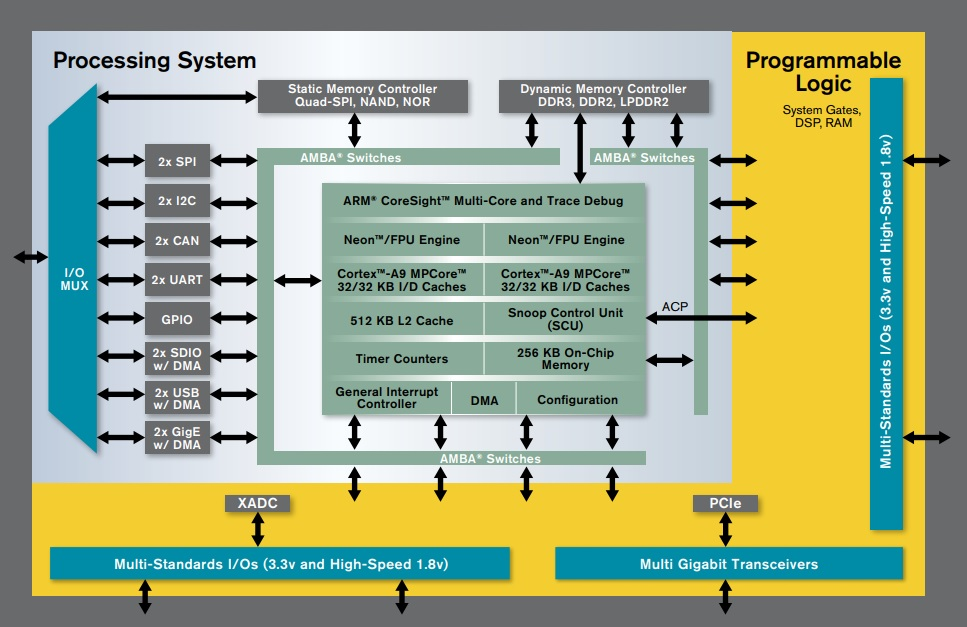
\includegraphics[width=0.9\textwidth]{zynq-pl-ps.jpg}
\end{frame}

\begin{frame}\frametitle{Zynq VHDL demo}
\centering
Let's try to run a simple VHDL example on the Zynq board. 
\end{frame}

\subsection{Pynq}

\begin{frame}\frametitle{Pynq}
Pynq is a project that provides a Python-based framework
for developing applications on Zynq-based FPGAs. \\
\vspace{0.5cm}
It allows users to write Python code that can interact 
with the FPGA fabric, enabling the development of 
hardware accelerators and other custom logic directly
usable in Python. \\
\vspace{0.5cm}
Pynq also provides a set of pre-built overlays,
which are pre-configured FPGA designs that can be used
to accelerate specific applications, such as image
processing or machine learning. \\
\end{frame}

\begin{frame}\frametitle{Pynq}

With this kind of technology, FPGAs are not anymore 
just a hardware platform, but they can be used as
computing accelerators in a high-level programming
language like Python. \\
\vspace{0.7cm}
With the term co-design, we mean the process of
developing both hardware and software components
together, taking advantage of the strengths of both
domains. \\
\vspace{0.7cm}
In the pynq \href{https://www.pynq.io/}{website},
(\href{https://www.pynq.io/}
{\textbf{https://www.pynq.io/}})
you can find a lot of examples
and tutorials to get started with Pynq and Zynq-based
FPGAs. 
\end{frame}

\begin{frame}\frametitle{Pynq}
Pynq is also available on the cloud environment,
let's see an example of how to use it. \\
\vspace{1cm}
in the day3/pynqExamples directory you can find
the Jupyter notebook and an example of co-design
in c++ as well.
\end{frame}

\subsection{Alveo}

\begin{frame}\frametitle{Alveo}
Alveo is a family of high-performance FPGAs designed 
for data center applications. \\
\vspace{1cm}
\centering
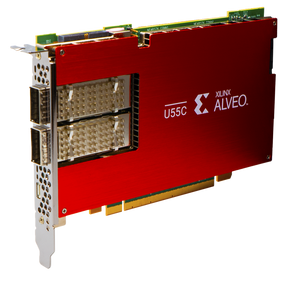
\includegraphics[width=0.5\textwidth]{alveou55c.png}
\end{frame}

\begin{frame}\frametitle{Alveo U55C}
\begin{table}[ht]
\centering
\fontsize{6}{7.2}\selectfont
\begin{tabular}{|l|p{3.5cm}|p{3.5cm}|}
\hline
\textbf{Feature} & \textbf{Xilinx Alveo U55C} & \textbf{Digilent Arty A7} \\
\hline
FPGA Family & Xilinx Virtex UltraScale+ HBM & Xilinx Artix-7 \\
\hline
FPGA Model & XCU55CHBVAU58P & XC7A35T or XC7A100T \\
\hline
Process Technology & 16nm FinFET & 28nm planar CMOS \\
\hline
Logic Resources (LUTs) & \textasciitilde1.3 million & 33,650 (A7-35T) / 101,440 (A7-100T) \\
\hline
Block RAM & 70.6 Mb + 8 GB HBM & 1.8 Mb \\
\hline
DSP Slices & 3,744 & 90 (A7-35T) / 240 (A7-100T) \\
\hline
HBM (High Bandwidth Memory) & 8 GB HBM2 & None \\
\hline
Memory Bandwidth & Up to 460 GB/s & Limited to external SRAM/DDR \\
\hline
Connectivity & PCIe Gen4 x16 & USB-UART, PMOD, Arduino headers \\
\hline
Power Consumption & High (server-grade, \textgreater 75W typical) & Low (\textasciitilde1--5W) \\
\hline
Form Factor & Full-height, full-length PCIe card & Standalone board (Arduino-style) \\
\hline
Typical Applications & Data center, HPC, AI, hardware acceleration & Education, prototyping, hobbyist projects \\
\hline
Approx. Price (2025) & \textgreater €10,000 & \textasciitilde €150--250 \\
\hline
Software Support & Vitis, Vivado, XRT, OpenCL & Vivado, Vitis (for optional MicroBlaze) \\
\hline
Host Requirements & Server/workstation with PCIe x16 slot & None (USB/UART for debugging) \\
\hline
Availability & Specialized enterprise resellers & Widely available online \\
\hline
\end{tabular}
\caption{Comparison between Xilinx Alveo U55C and Digilent Arty A7}
\label{tab:fpga_comparison}
\end{table}
\end{frame}

\begin{frame}\frametitle{HLS}
Board like the Alveo U55C are used in data centers, so 
FPGAs are not only used for prototyping or for electronics
projects, but start to be used in high-performance computing
and in data centers. \\
\vspace{1.5cm}
Concurrently to this shift in the use of FPGAs, there is also a
shift in the way to program them. The development
of High-Level Synthesis (HLS) tools allows developers to
write code in high-level programming languages like C, C++,
or OpenCL, which is then translated into hardware description
languages (HDL) like Verilog or VHDL. \\
\end{frame}

\end{document}

